%%%%%%%%%%%%%%%%%%%%%%%%%%%%%%%%%%%%%%%%%
% Stylish Article
% LaTeX Template
% Version 2.1 (1/10/15)
%
% This template has been downloaded from:
% http://www.LaTeXTemplates.com
%
% Original author:
% Mathias Legrand (legrand.mathias@gmail.com) 
% With extensive modifications by:
% Vel (vel@latextemplates.com)
%
% License:
% CC BY-NC-SA 3.0 (http://creativecommons.org/licenses/by-nc-sa/3.0/)
%
%%%%%%%%%%%%%%%%%%%%%%%%%%%%%%%%%%%%%%%%%

%----------------------------------------------------------------------------------------
%	PACKAGES AND OTHER DOCUMENT CONFIGURATIONS
%----------------------------------------------------------------------------------------

\documentclass[fleqn,12pt]{SelfArx_ch} % Document font size and equations flushed left

\usepackage[english]{babel} % Specify a different language here - english by default

\usepackage{lipsum} % Required to insert dummy text. To be removed otherwise

\captionsetup[figure]{justification=justified, singlelinecheck=off} 
\captionsetup[table]{justification=justified, singlelinecheck=off} 

%----------------------------------------------------------------------------------------
%	COLUMNS
%----------------------------------------------------------------------------------------

\setlength{\columnsep}{0.55cm} % Distance between the two columns of text
\setlength{\fboxrule}{0.75pt} % Width of the border around the abstract
\linespread{1.5}

%----------------------------------------------------------------------------------------
%	COLORS
%----------------------------------------------------------------------------------------

\definecolor{color1}{RGB}{0,0,90} % Color of the article title and sections
\definecolor{color2}{RGB}{10,20,20} % Color of the boxes behind the abstract and headings
\definecolor{xsubj}{RGB}{243,194,68} 
\definecolor{xsess}{RGB}{53,99,161} 
\definecolor{xsamp}{RGB}{18,165,121} 

%----------------------------------------------------------------------------------------
%	HYPERLINKS
%----------------------------------------------------------------------------------------

\usepackage{hyperref} % Required for hyperlinks
\hypersetup{hidelinks,colorlinks,breaklinks=true,urlcolor=color2,citecolor=color1,linkcolor=color1,bookmarksopen=false,pdftitle={Title},pdfauthor={Author}}
%----------------------------------------------------------------------------------------
%	ARTICLE INFORMATION
%----------------------------------------------------------------------------------------

% \JournalInfo{Journal, Vol. XXI, No. 1, 1-5, 2013} % Journal information
\JournalInfo{$ $ }
\Archive{ }
\PaperTitle{Ch.II: Comparing Perturbation Models for Evaluating Stability of Neuroimaging Pipelines}
\Authors{Gregory Kiar\textsuperscript{1}, Pablo de Oliveira Castro\textsuperscript{2},
Pierre Rioux\textsuperscript{1}, Eric Petit\textsuperscript{3}, Shawn T. Brown\textsuperscript{1},
Alan C. Evans\textsuperscript{1}, Tristan Glatard\textsuperscript{4}} % Authors
\affiliation{\textsuperscript{1}\textit{Montréal Neurological Institute, McGill University, Montréal, QC, Canada}}
\affiliation{\textsuperscript{2}\textit{University of Versailles, Versailles, France}}
\affiliation{\textsuperscript{3}\textit{Exascale Computing Lab, Intel, Paris, France}}
\affiliation{\textsuperscript{4}\textit{Department of Computer Science and Software Engineering, Concordia University, Montréal, QC, Canada}}

%----------------------------------------------------------------------------------------
%	ABSTRACT
%----------------------------------------------------------------------------------------

\Abstract{With an increase in awareness regarding a troubling lack of reproducibility in analytical software tools, the
degree of validity in scientific derivatives and their downstream results has become unclear. The nature of
reproducibility issues may vary across domains, tools, datasets, and computational infrastructures, but numerical
instabilities are thought to be a core contributor. In neuroimaging, unexpected deviations have been observed when
varying operating systems, software implementations, or adding negligible quantities of noise. In the field of
numerical analysis these issues have recently been explored through Monte Carlo Arithmetic, a method involving the
instrumentation of floating point operations with probabilistic noise injections at a target precision. Exploring
multiple simulations in this context allows the characterization of the result space for a given tool or operation. In
this paper we compare various perturbation models to introduce instabilities within a typical neuroimaging pipeline,
including i) targeted noise, ii) Monte Carlo Arithmetic, and iii) operating system variation, to identify the
significance and quality of their impact on the resulting derivatives. We demonstrate that even low-order models in
neuroimaging such as the structural connectome estimation pipeline evaluated here are sensitive to numerical
instabilities, suggesting that stability is a relevant axis upon which tools are compared, alongside more traditional
criteria such as biological feasibility, computational efficiency, or, when possible, accuracy. Heterogeneity was
observed across participants which clearly illustrates a strong interaction between the tool and dataset being
processed, requiring that the stability of a given tool be evaluated with respect to a given cohort. We identify use
cases for each perturbation method tested, including quality assurance, pipeline error detection, and local sensitivity
analysis, and make recommendations for the evaluation of stability in a practical and analytically-focused setting.
Identifying how these relationships and recommendations scale to higher-order computational tools, distinct datasets,
and their implication on biological feasibility remain exciting avenues for future work.}

%----------------------------------------------------------------------------------------

\begin{document}
\flushbottom % Makes all text pages the same height
\maketitle % Print the title and abstract box
\thispagestyle{empty} % Removes page numbering from the first page
\clearpage
\makeabstract

\onecolumn 
\beginchapter{II}
%----------------------------------------------------------------------------------------
%	ARTICLE CONTENTS
%----------------------------------------------------------------------------------------
\section{Introduction}
A lack of computational reproducibility~\cite{Peng2011-cz} has become increasingly apparent in the last several years,
calling into question the validity of scientific findings affected by published tools. Reproducibility issues may have
numerous sources of error, including undocumented system or parametrization differences and the underlying numerical
stability of algorithms and implementations employed. While containerization can mitigate the extent of
machine-introduced variability, understanding the effect that these sources of error have on the encapsulated numerical
algorithms remains difficult to explore. In simple cases where algorithms are differentiable or invertible, it is
possible to obtain closed-form solutions for their stability. However, as software pipelines grow, containing multiple
complex steps, using non-linear optimizations and non-differentiable functions, the stability of these algorithms must
be explored empirically.

As neuroscience has evolved into an increasingly computational field, it has suffered from the same questions of
numerical reproducibility as many other domains~\cite{Baker2016-en}. In particular, neuroimaging often attempts to fit
alignments, segmentations, or models of the brain using few samples with variable signal to noise properties. The
nature of these operations leaves them potentially vulnerable to instability when presented with minor perturbations in
either the data themselves or their processing implementations. The independent evaluation of atomic pipeline
components may be feasible in some cases, as was done by Skare et al. in \cite{Skare2000-sl}. Here, the authors
computed the theoretical conditioning of various tensor models used in diffusion modeling, and compared these values to
the observed variances in tensor features when fit on simulated data. While approaches like the above provide valuable
insights to algorithms and their implementations independently, the impact of these stepwise instabilities within
composite pipelines remains unknown. Even if one were able to evaluate each step within a pipeline, identifying the
impact these instabilities may have on a result when composed together, both structurally and analytically, remains
practically difficult to evaluate. Additionally, as datasets grow in size, the adoption of High Performance Computing
environments becomes a necessity. These environments are highly heterogeneous in terms of hardware, operating systems,
and parallelization schemes, and this heterogeneity has been shown to compound with these instabilities and impact
results~\cite{Glatard2015-vc}.

Various forms of instability have been observed in structural and functional magnetic resonance (MR) imaging, including
across operating system versions~\cite{Glatard2015-vc}, minor noise injections~\cite{Lewis2017-ll}, as well as dataset
or implementation of theoretically equivalent algorithms~\cite{Bowring2018-ed,Klein2009-bl}. These approaches may have
practical applications in decision making, such as deciding which tool/implementation should be used for an experiment.
However, they are relatively far removed from the underlying numerical instabilities being observed. Recent advances in
numerical analysis allow for the replacement of floating point operations with Monte Carlo Arithmetic
simulations~\cite{Parker1997-qq} which inject a random zero-bias rounding error to operations for a target
floating-point precision~\cite{Parker1997-qq, Frechtling2015-cd}. This method can be used for evaluating the numerical
stability of tools by wrapping existing analyses~\cite{Frechtling2015-cd} and providing a foothold for scientists
wishing to explore the space of their pipeline's compound instabilities~\cite{Denis2016-wo}.

In this paper we explore the effect of various perturbations on a typical diffusion MR image processing pipeline
through the use of i) targeted noise injections, ii) Monte Carlo Arithmetic, and iii) varying operating systems to
identify the quality and severity of their impact on derived data. This evaluation will inform future work exploring
the stability of these pipelines and downstream analyses dependent upon them. The processing pipeline selected for
exploration is Dipy~\cite{Garyfallidis2014-ql}, a popular tool that generates structural connectivity maps
(connectomes) for each participant. The pipeline accepts de-noised and co-registered images as inputs, and then
performs two key processing steps: tensor fitting and tractography. We demonstrate the relative impact that each of the
tested perturbation methods has on the resulting connectomes and explore the nature of where these differences emerge.

\section{Methods}
All processing described below was run using servers provided by Compute Canada. Software pipelines were encapsulated
and run using Singularity~\cite{Kurtzer2017-kq} version 2.6.1. Tasks were submitted, monitored, and provenance captured
using Clowdr~\cite{kiar2019-clowdr} version 0.1.2-1. All code for performing the experiments and creating associated
figures are available on GitHub at \href{https://github.com/gkiar/stability}{https://github.com/gkiar/stability} and
\href{https://github.com/gkiar/stability-mca}{https://github.com/gkiar/stability-mca}, respectively.

\subsection{Dataset and pre-processing}
The dataset used for processing is a 10-session subset of the Nathan Kline Institute Rockland Sample dataset
(NKI-RS)~\cite{Nooner2012-eg}. This dataset contains high fidelity structural, functional, and diffusion MR data and is
openly available for research consumption. The $10$ sessions used were chosen by randomly selecting $10$ participants
and selecting their alphabetically-first session of data. This data was preprocessed prior to the modelling evaluated
here using a standard de-noising and image alignment pipeline~\cite{Greg_Kiar2019-ds} built upon the FSL
toolbox~\cite{Jenkinson2012-ly}. The steps in this pipeline include eddy current correction, brain extraction, tissue
segmentation, and image registration. The boundary between white and gray matter was obtained by computing the
difference between a dilated version of the white matter mask and the original. Data volumes at this stage of
processing are four-dimensional and variable in spatial extent (first three dimensions) with a fixed number of
diffusion directions (fourth dimension), totalling approximately $100^3 \times 137$ voxels in each case.

\subsection{Modeling}\label{sec:modeling}
After pre-processing the raw diffusion data using FSL, structural connectomes were generated for an $83$-region
cortical and sub-cortical parcellation~\cite{Cammoun2012-yw} using Dipy~\cite{Garyfallidis2014-ql}. A
six-component tensor model was fit to the diffusion data residing within white matter. Seeds were generated in a
$2 \times 2 \times 2$ arrangement for each voxel within the boundary mask, resulting in 8 seeds per boundary voxel.
Deterministic tracing was then performed using a half-voxel step size, and streamlines shorter than $3$-points in
length were discarded as spurious. Once streamlines were generated they were traced through the parcellation. Edges
were added to the graph corresponding to the end-points of each fiber, and were weighted by the streamline count. This
pipeline was implemented in Python, including a few components in Cython, and relies on the Numpy library for a large
proportion of operations. Each resulting network is a square connectivity matrix of $83 \times 83$ edges, as shown in
Fig.~\ref{fig1:example}. This pipeline was chosen as it is both common and simple relative to many alternatives.

\begin{figure}[t!]
\centerline{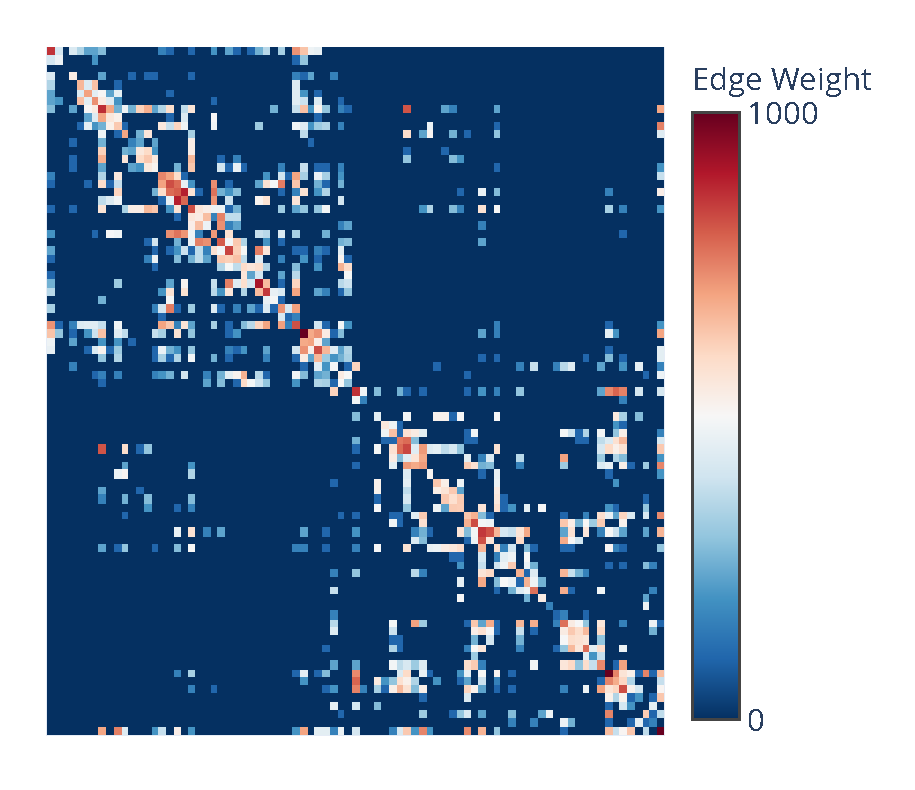
\includegraphics[width=\linewidth]{figures/fig1_example_graph.pdf}}
\caption{\textbf{Example connectome}. Each row and column corresponds to a region
within the brain, and the intersection a connection between them. If no connection
is found between regions, the edge strength is zero. If a streamline is found to
connect two regions, the weight is incremented by $1$. The resulting weights are
the sum of all observed connections for every streamline traced within a brain image.}
\label{fig1:example}
\end{figure}

\subsection{Stability Evaluation}
Targeted and Monte Carlo perturbation modes were tested 100x per image. Noise was represented by percent deviation of
the Frobenius norm of a resulting connectome from the corresponding reference (no noise injection). A deviation of
$50 \%$ indicates that the norm of the difference between the noisy and reference networks is $50 \%$ the size of the
norm of the reference graph. This is formalized below in Eq.~\eqref{eq:eval}:

\begin{equation}
\% Dev (A, B) = \sqrt{\sum_{i=1}^m\sum_{j=1}^n \lvert a_{ij} - b_{ij} \rvert^2 } / \sqrt{\sum_{i=1}^m\sum_{j=1}^n \lvert a_{ij} \rvert^2},
\label{eq:eval}
\end{equation}

where $A$ is the reference graph, $B$ is the perturbed graph, and $\square_{ij}$ is an element therein at row $i$ and
column $j$.

The perturbation methods evaluated, presented below, are summarized in Table~\ref{tab1}.

\subsection{Subject-Level Variation}
Comparison between subjects will be used as a reference error. If the differences observed by other methods are similar
in magnitude to the subject-level difference, then the validity of the processed networks for use in downstream
phenotypic analysis becomes questionable as subjects cannot be reliably distinguished from one another. This error is
computed as the pairwise distance between all $10$ subjects included in this cohort.

\subsection{Targeted Noise}
The goal of targeted noise was to inject data perturbations sufficiently small that the resulting images would be
indistinguishable from the original. This is meant to test the lower-bound of noise sensitivity for processing
pipelines. The type of targeted noise used here will be referred to as $1$-voxel noise and is similar to the method
employed in~\cite{Lewis2017-ll}. In our case, the intensity of a single voxel in the defined range will be scaled based
on a scaling factor. The voxels modified in this case were randomly generated within the mask of brain regions being
modeled by the pipeline.

The two modes of $1$-voxel noise injection tested here were: a) a single voxel per entire image of size $(X, Y, Z, D)$
(approximately $100^3 \times 137$ for all images), or b) a single voxel per $3$D volume of size $(X, Y, Z)$
(approximately $100^3$ for all images), and are referred to as ``single'' and ``independent'' modes, respectively.
While the number of perturbed voxels in the independent case is approximately 100 times larger, the intensity of
magnification was consistent as in both cases the original voxel intensities were doubled.

\subsection{Monte Carlo Arithmetic}
Verificarlo~\cite{Denis2016-wo} is an extension of the LLVM compiler which automatically instruments floating point
operations at build-time for software written in C, C++, and Fortran. Once compiled with Verificarlo, the Monte Carlo
emulation method and target precision can be set as environment variables. For all simulations a rounding error on the
least significant floating point bit in the mantissa (bit $53$) was introduced. The simulations were computed using the
custom QUAD backend which is optimized to reduce computation time over the traditional mcalib MPFR backend leveraging
GNU’s multiple precision library~\cite{Frechtling2015-cd}. Noise through Verificarlo can be injected as ``Precision
Bounded'', simulating floating point cancellations, ``Random Rounding'', simulating only rounding errors on
computation, and ``MCA'', which includes both of these modes. A particularity of the Random Rounding mode is that it
only injects rounding noise on inexact floating-point operations (i.e. operations that have a rounding error in
IEEE-754 at the target precision). Therefore, RR mode preserves the original exact operations, it is a more
conservative noise simulation. We used both the RR and MCA modes of simulation.

Verificarlo was used to instrument tools in two modes we will refer to as ``Python'' and ``Full Stack''. In the Python
instrumentation, the core Python libraries were recompiled with Verificarlo as well as any subsequently installed
Cython libraries. In the Full Stack instrumentation, BLAS and LAPACK were also recompiled, meaning that Numpy, a
dominant Python library for linear algebra, was also instrumented. The Full Stack implementation did not run
successfully using the MCA mode. We suspect that some libraries require exact floating-point operations or are
sensitive to cancellation errors, so only the Random Rounding (RR) mode was able to be evaluated for the Full Stack.
These instrumentations took approximately 10 hours for the authors to refine, and the images are available on DockerHub
at gkiar/fuzzy-python.

\begin{table}[b!]
    \caption{Description of perturbation modes}
    \begin{center}
    \begin{tabular}{p{0.15\linewidth} p{0.75\linewidth}}
    \textbf{Permutation} & \textbf{Description} \\
    \hline
    X-Subject &
    Pairwise comparison of sessions based on \textbf{Subject ID}.
    \\
    $1$-voxel &
    Intensity value doubled for either \textbf{Single} (one voxel in entire
    $4$D volume) or \textbf{Independent} (one voxel per $3$D sub-volume) voxels.
    \\
    MCA &
    Simulation of all floating point operations in \textbf{Python} (Python and
    Cython-compiled libraries).
    \\
    RR &
    Simulation of all rounding operations in \textbf{Python} or the
    \textbf{Full Stack} (BLAS, and LAPACK, Python and Cython-compiled libraries).
    \\
    X-OS &
    One of \textbf{Ubuntu 16.04} or \textbf{Alpine 3.7.1}.
    \end{tabular}
    \label{tab1}
    \end{center}
\end{table}

\subsection{Operating System Variation}
Operating system noise was evaluated across Alpine Linux 3.7.1 and Ubuntu 16.04. Alpine is a lightweight distribution
which comes with minimal packages or libraries, and Ubuntu is a popular Linux distribution with a large user and
development community. Alpine was chosen as its lightweight nature makes it an efficient choice for the packaging and
distribution of libraries in containers for scientific computing, reducing the overhead of shipping code towards data
sources. Ubuntu was chosen due to is high adoption and community support by major libraries. While Alpine comes with a
minimal set of libraries, a core difference between these systems as noted by DistroWatch
(\href{https://distrowatch.com/}{https://distrowatch.com/}) is their dependence on a different version of the Linux
kernel. While numerical differences between operating systems are likely the result of compilers~\cite{sawaya2017flit}
and installed libraries, the purpose of testing across operating systems explicitly rather than combinations of
specific tools is to re-create a real-world setting in which typical scientific users observe numerical differences
across equivalent high-level pipelines.

Ubuntu was used as the base operating system for all simulations other than this comparison. The variability observed
across operating systems was  aggregated across participants and included as a reference margin of error.

\begin{figure*}[bth!]
\centerline{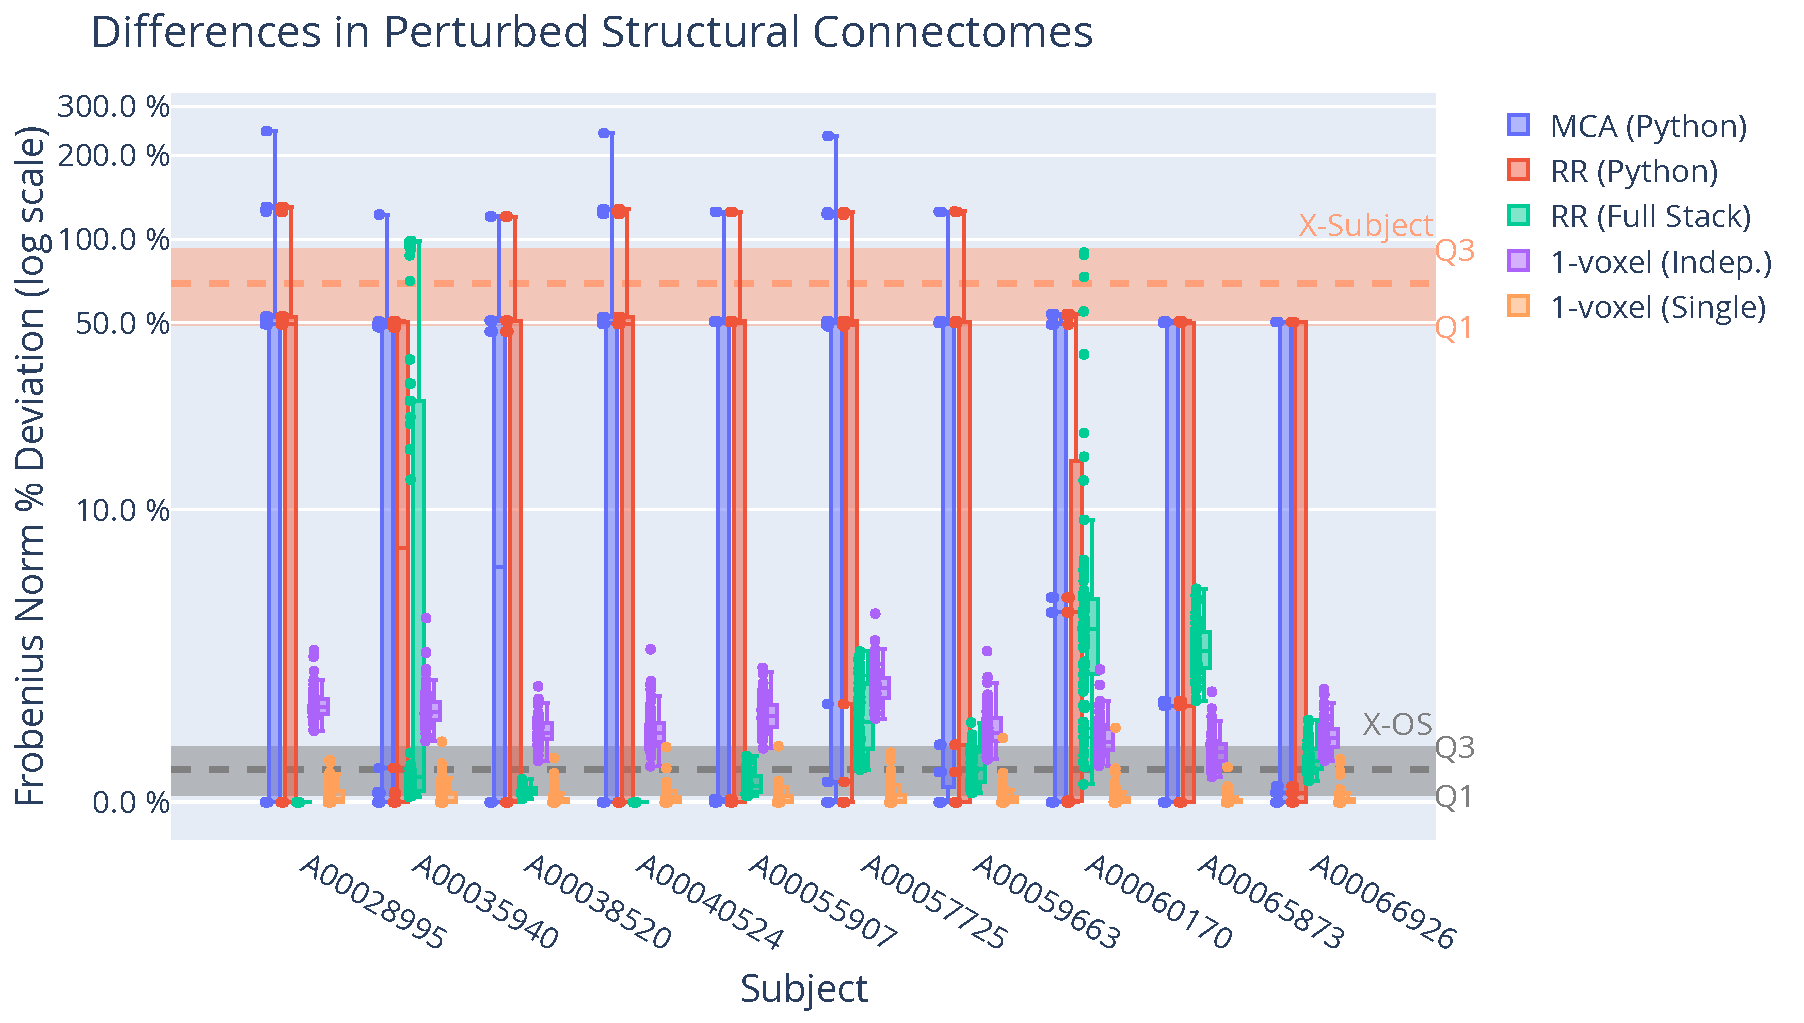
\includegraphics[width=1.1\textwidth]{figures/fig2_fro_summary.pdf}}
\caption{\textbf{Comparison of perturbation modes}. As evaluated by the percent
deviation from reference in the Frobenius Norm of a resulting connectome, each
of the $10$ processed subjects were re-processed $100$ times for each perturbation
method. We see that the MCA and RR (Python) methods resulted in distinct modes
for the outputs in all cases reaching extreme deviations equivalent to cross-subject
variation. The RR (Full Stack) method shows high variability across subjects, and
only reaching cross-subject variation in the case of $2$ subjects. The $1$-voxel
methods result in considerably less deviation from reference, and are more consistent
across subjects than the RR (Full Stack) method.}
\label{fig2:summary}
\end{figure*}

\subsection{Aggregation of Simulated Graphs}
To structurally evaluate each simulation setting, connectomes were aggregated within setting and subject combinations.
Several aggregation methods were explored to preserve various sensitivity and stability properties across the
aggregated graphs. In each case, the operations are performed edge-wise, so the aggregated graph is not guaranteed to
be single graph in the set of perturbed graphs. The aggregation operations are the edge-wise mean and the $0^{th}$
(min), $10^{th}$, $50^{th}$ (median), $90^{th}$, and $100^{th}$ (max) $\%$-iles. The mean aggregate will include a
non-zero weight for every edge which appears in at least one simulation, and the $0^{th}$ and $100^{th}$ \%-iles will
include the lowest and highest observed weight for every edge, respectively. The $90^{th}$, $50^{th}$, and $10^{th}$
\%-iles increasingly aggressively filter edges based on their prominence across simulations. The combination of
percentile aggregates also enable isolation of the most spurious edges, such as by taking the difference of maximum and
minimum aggregates. A volatile aggregate was created to this effect which consists of edges which are found in the
maximum aggregate but not the minimum aggregate. Note that in this case, the weight for these edges is not implied and
can be defined as an alternative function of the graph collection, such as mean, but as the weight does not appear when
comparing binary edges, no recommendation for this weighting is made here.

\section{Results}
\label{sec:res}
All perturbation modes were applied to either the input data or post-processing pipeline described in the
Section~\ref{sec:modeling}, and were evaluated according to Eq.~\eqref{eq:eval}.

\subsection{Perturbation Induced Differences}
Fig.~\ref{fig2:summary} shows the percentage deviation for each simulation mode on 10 subjects. Introduced
perturbations show highly-variable changes in resulting connectomes across both the perturbation model and subject,
ranging from no change to deviations equivalent to difference typically observed across subjects. For the $10$ subjects
tested, we see that the Python-instrumented MCA and RR pipelines resulted in the largest deviation from the reference
connectome. In these cases we also see that the results are modal, where each subject has discrete states that may be
settled in, some of which result in deviations comparable to subject-level noise. This modality is likely due to minor
differences introduced at crucial branch-points which then cascaded throughout the pipeline. This hypothesis is
supported by observing that the Full Stack implementation with RR perturbations shows a continuous distribution of
differences that are highly variable in intensity, ranging from no deviation to subject-level in some cases for some
subjects, which are explored in Section~\ref{sec:progdev}.

The $1$-voxel independent mode unsurprisingly produces larger changes than the $1$-voxel single mode. These changes are
larger than or comparable to operating system variability, respectively, resulting in small deviations from the
reference, and are relatively minor in comparison to the extremes observed with Monte Carlo Arithmetic. Operating
system deviations are very low or even zero in some cases. In all perturbation settings we can see that there is large
variability both across simulations on the same data and across subjects.

\subsection{Progression of Deviations in a Continuous Setting}
\label{sec:progdev}

In the case of subject A00035940, the Full Stack RR perturbations led to a continuous distribution of outputs, ranging
in difference from none to subject-level from the reference. Fig.~\ref{fig3:exploration} explores the progression of
these deviations by visualizing the difference-connectome for samples along various points of this distribution. In the
center we show the reference connectome, and surrounding it the difference graph for a simulated sample with labelled
$\% Dev$ from this reference. In this case, we can see a progression of structurally consistent deviations. In
particular, edges corresponding to regions in the left hemisphere become increasingly distorted (bottom-right portion
of the connectome), whereas the within-hemisphere connectivity for the right hemisphere (top-left portion) remains
largely intact in all cases except the extreme difference case. We notice in all cases that the connectivity between
regions is decreasing until the edges disappear entirely. While this behaviour is not consistent across all subjects,
this observation suggests a peculiarity in the quality of data in this region for the subject in question. This could
be due to artifacts caused by motion or other factors, ultimately reducing the stability of modeling connectivity in
this region.

\begin{figure}[t!]
    \centerline{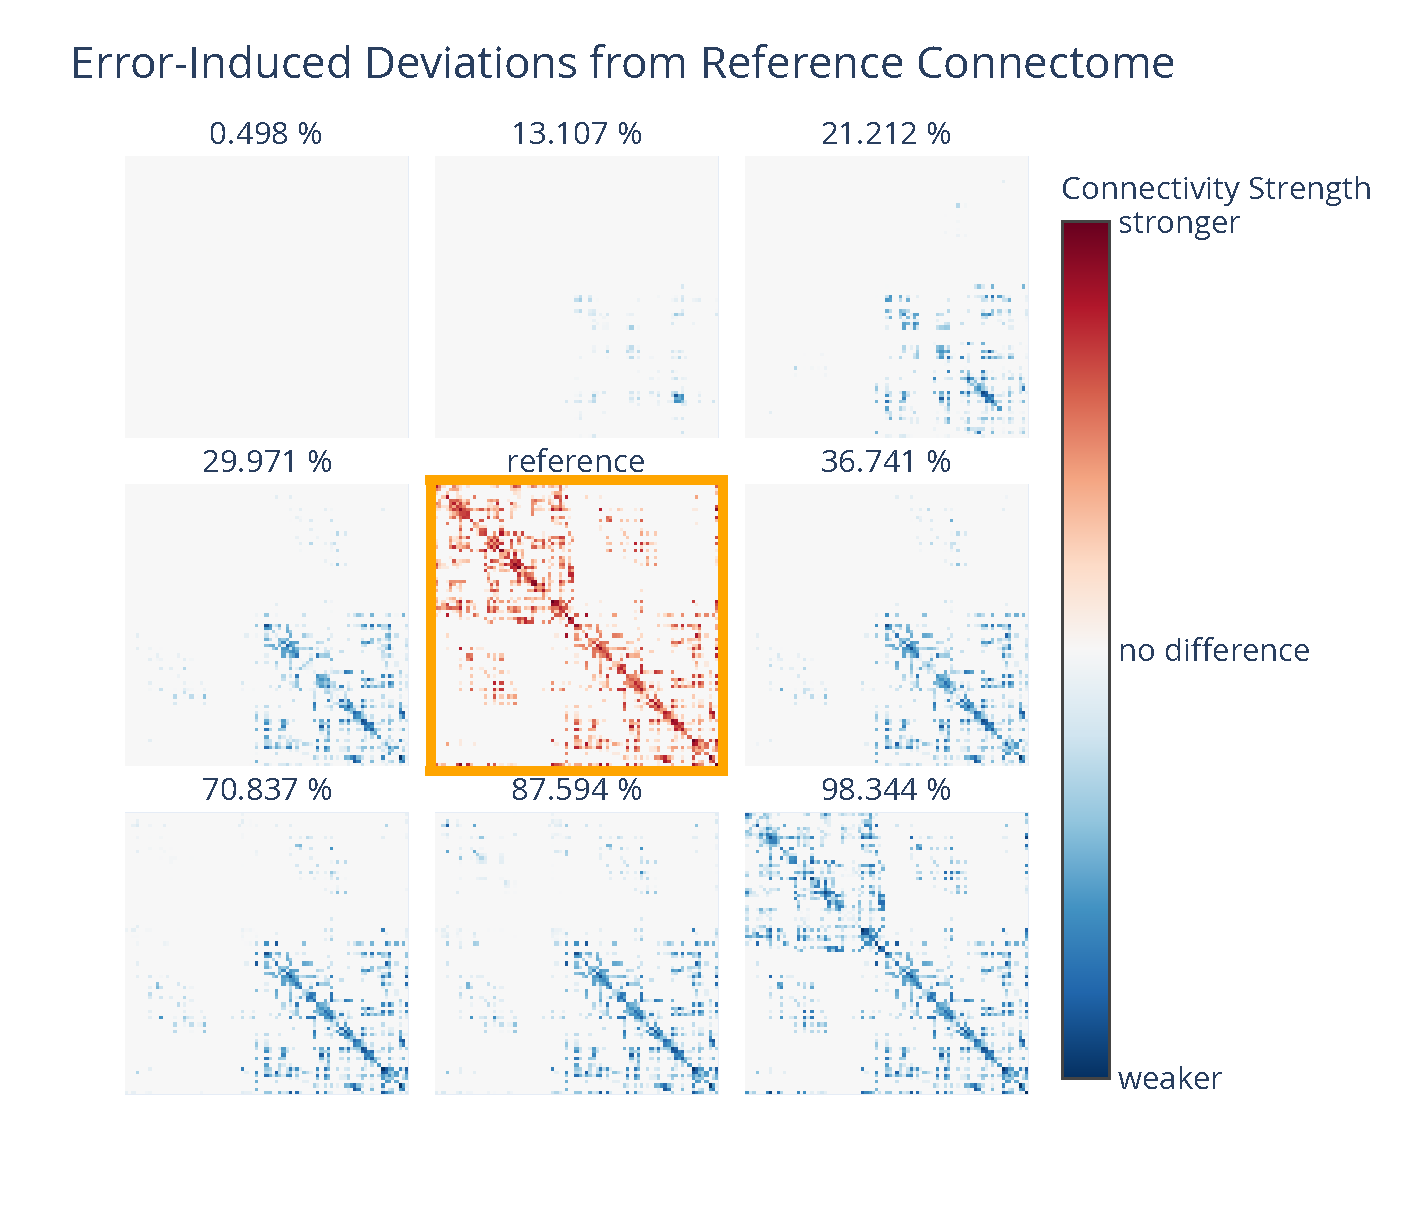
\includegraphics[width=\linewidth]{figures/fig3_fro_A00035940_panel.pdf}}
\caption{\textbf{Structure of Deviations}. Shown in increasing deviation from
left--right and top--bottom, with the reference in the centre, are the difference
connectomes observed for the RR (Full Stack) perturbations of subject A00035940.
In this case, the left hemisphere (bottom-right portion of the graph) begins to
degrade quickly, eventually reaching an almost complete loss in signal.}
\label{fig3:exploration}
\end{figure}

\subsection{Structural Properties of Introduced Perturbation}
While the case investigated above notably showed a significant degradation of regional signal quality for Full Stack RR
noise in a single subject, Fig.~\ref{fig4:structural_variances} explores the relative change in connectivity from the
reference for each perturbation mode and subject. Edges in the presented graphs are weighted by their standard
deviation across all simulations for that participant, and coloured as positive or negative deviations based on whether
the mean weight for all simulations was greater or lower than the reference weight, respectively. All edges with a
standard deviation of $0$ across all simulations were greened out for clarity.

For the Python instrumented MCA and RR implementations, edge weight was generally inflated non-specifically for
existing edges in the reference connectome for all subjects. The Full Stack RR implementation shows significant
variability across subjects, where the number of affected edges ranges from none to all. In each case where there
exists some deviation, intensities appear to be spatially linked, suggesting the differences may be due to variable
quality in the underlying data. In this case, Monte Carlo Arithmetic may have served to shed light on poor
signal-to-noise properties present within regions of the images being modelled.

For $1$-voxel noise, the differences introduced across independent injections impacted a larger portion of edges than
single injections, unsurprisingly. By design (i.e. injection at random locations for each simulation), the deviations
appear non-specifically spatially distributed. However, $1$-voxel noise could be modified to spatially constrain the
location for noise injection regionally, allowing the evaluation of modelling for particular sub-structures within the
images.

\subsection{Aggregation Across Simulations}

For each simulation method there existed a graph nearly identical to the reference, but the variability introduced by
these simulations were highly variable both in terms of the method of perturbation used and the dataset being
processed. The aggregation of the simulated graphs into a consensus graph allows features of this variation to be
encoded implicitly in connectomes which may be used for downstream analyses. Fig.~\ref{fig5:aggregation_methods} shows
the relative percentage of added and missing edges for each setting across all subjects using a variety of such
aggregation methods.

\begin{figure*}
    \centerline{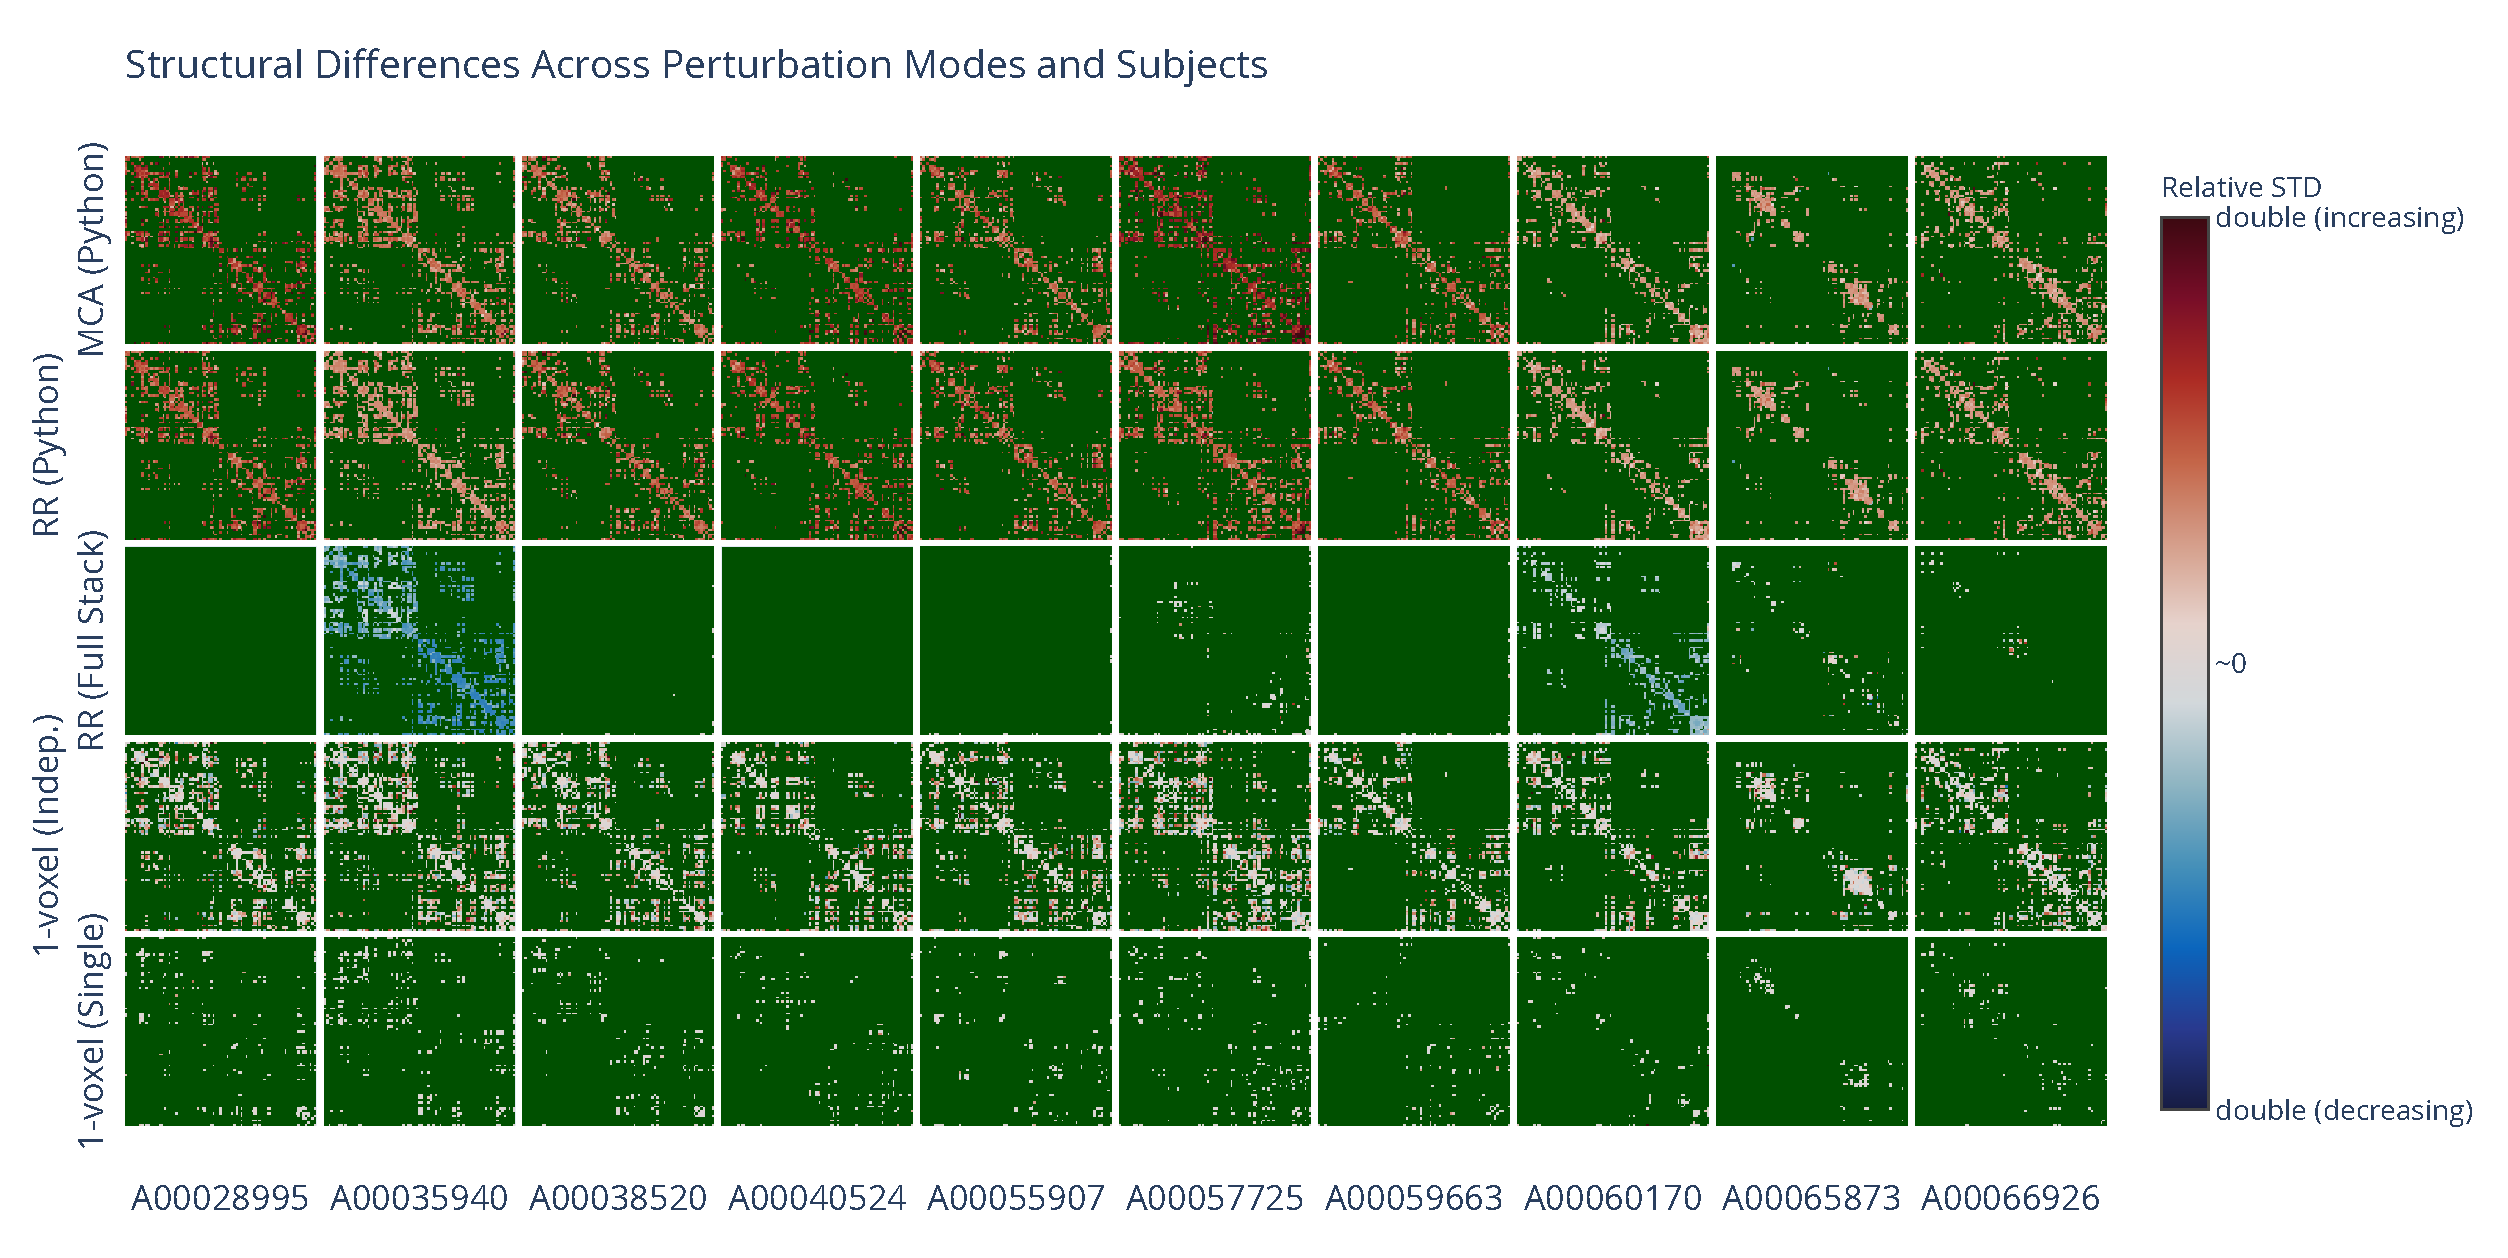
\includegraphics[width=1.1\linewidth]{figures/fig4_directed_variance_structure_panel.pdf}}
    \caption{\textbf{Perturbation introduced structural differences}. The variance
    of each edge is shown relative to the reference edge strength, and coloured
    either red or blue based on the mean perturbed weight was higher or lower than
    that of the reference, respectively. Edges which experienced no variation were
    coloured as green to be distinct from all edges which experience any variation.}
    \label{fig4:structural_variances}
\end{figure*}

By aggregating the simulated connectomes in a variety of methods, the resulting edges would be a product of applying
some filter to the set of observed edges, and succinctly represented in a single graph. While minor deviations in one
edge may reduce the strength of connectivity between two strongly linked regions, the addition of a connection between
two regions which were previously unconnected may be significant in one aggregation method but ignored in another. In
the case of the above example, despite the strength of connectivity remaining low between the newly connected nodes
many graph theoretic measures rely on binarized graphs and may be considerably affected, such as the degree.

We notice that the $1$-voxel independent (i.e. single voxel per $3$D volume) method shows the most variability across
each aggregation method. Where all of the MCA-derived methods perturb the pipeline non-locally, both epsilon-level
methods add local noise at arbitrary locations. This distinction seems to manifest in more widely added or knocked-out
edges for the $1$-voxel cases, as the location of noise may have considerable impact on a multitude of nearby fibers,
where MCA methods have a zero-bias noise globally, meaning all deviations from the reference are spurious and due to
numerical error rather than the introduction of a systemic change that sheds light on an underlying cascading
instability.

Unsurprisingly, the only aggregation method which shows considerable amount of both new and missing edges is the
volatile technique, which takes edges that exist in the binary difference of $100^{th}$ and $0^{th}$ percentile graphs,
eliminating all extremely stable edges from the graph (i.e. those which exist for the reference and all simulations).
While the mean sparsity of the reference graphs is $0.30$, meaning $30 \%$ of possible connections have non-zero weight
on average, the sparsity of the volatile aggregates ranges from $0.005$ to $0.130$, or, the aggregates contain between
$2.5 \%$ and $43.0 \%$ the number of edges as the reference graphs. 

\subsection{Comparison of Simulation Performance}
While the application of each perturbation model tested sheds light on different properties of pipeline stability, the
resource consumption of these methods has significant bearing when processing data in the context of a real experiment
often consisting of dozens to hundreds of subjects worth of data. In this experiment, a single unperturbed pipeline
execution took approximately $20$ minutes using $1$ core and $6$ GB of RAM. Fig.~\ref{fig5:timing} shows the relative
Time-on-CPU for a single simulation of each method tested, relative to the reference task with no instrumentation. For
Monte Carlo Arithmetic instrumented executions, we expect to see a considerable increase in computation time as
additional overhead is added to each floating point operation. In the case of $1$-voxel noise it is expected to see a
minor increase in computation time as the perturbed data volumes were generated at runtime, reducing the data
redundancy on disk. 

The Python MCA and RR modes show a slight increase in computation time to the reference task, whereas the Full Stack
version approaches a nearly $7 \times$ slowdown, on average. This discrepancy further supports the hypothesis stated
above that floating point logic implemented directly in Python, without the use of Numpy or external libraries, account
for a minor portion of the total floating point operations. As Verificarlo has been shown to increase the runtime of
floating point operations by approximately $100 \times$, this result suggests that the pipeline evaluated here is
largely I/O limited. In the case of $1$-voxel perturbations, we see a slowdown approximately equivalent to that of the
Python instrumentation, not exceeding a $2 \times$ increase. Across all executions approximately 2000 CPU~hours were
consumed. While this is a small workload in the context of HPC, the required resources quickly reach the order of
CPU~years after extrapolating to the entire NKI-RS dataset or others in neuroimaging.

\begin{figure*}[bth]
    \centerline{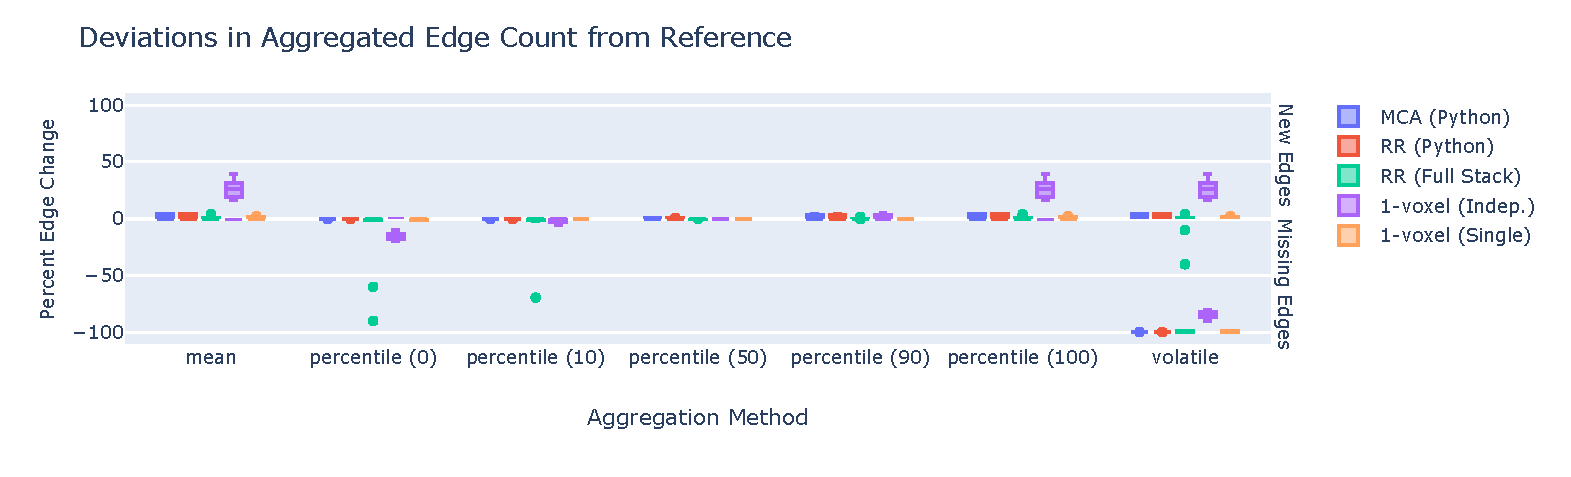
\includegraphics[width=1.1\linewidth]{figures/fig5_aggregation_methods.pdf}}
    \caption{\textbf{Gain and loss of edges in aggregation of simulations}.
    The relative gain and loss of edges is shown for each aggregation method and
    perturbation method in terms of binary edge count. The volatile aggregation
    is the difference between percentile ($100$) and percentile ($0$) aggregates,
    and is contains all edges which do not appear in every graph. The volatile
    set of edges for each of MCA (Python), RR(Python), RR (Full Stack),
    $1$-voxel (independent), and $1$-voxel (single) contain $2.5 \%$, $2.5 \%$,
    $18.5 \%$, $43.0 \%$, and $1.7 \%$ of the number of edges found in the
    reference, respectively. In the worst case, $1$-voxel (independent), this
    means that the existence of nearly half the edges in the graph fail to have
    consensus across the simulations.}
    \label{fig5:aggregation_methods}
\end{figure*}

\section{Discussion}
We have demonstrated through the application of multiple perturbation methods how noise can be effectively injected
into neuroimaging pipelines enabling the exploration and evaluation of the stability of resulting derivatives. These
methods operate by either perturbing the datasets or tools used in processing, resulting in a range of structurally
distinct noise profiles and distributions which may each provide value when exploring the stability of analyses. While
$1$-voxel noise is injected directly into the datasets prior to analysis, MCA and RR methods iteratively add
significantly smaller amounts of noise to each operation performed.

In the case of partial (Python) instrumentation with MCA and RR, distinct and considerably distinct modes emerged in
all tested subjects. We hypothesize that software branching likely played a role leading to this unexpected result. As
the majority of numerical analysis in Python is traditionally performed using the Numpy library, and therefore BLAS and
LAPACK, it is possible that the error introduced by Python was allowed to cascade throughout the pipeline without
correction, until the next Python branch point occured and this repeated, eventually growing to the often subject-level
differences observed. These modes would then be the result of a small number of instrumented numerically-sensitive
operations, leading to a bounded set of possible outcomes of an otherwise deterministic process. It is possible that
these distinct modes could serve as upper-bounds for the deviation due to instabilities within a pipeline, and is an
area for further exploration. Future work will also more closely instrument libraries with functionality that will
enable the identification of crucial branch points, as this functionality is already present within Verificarlo. The
identified crucial branch points could be leveraged for the re-engineering of pipelines with more stable behaviour,
and potentially shed light on new ``best practices''.

An exciting application of MCA and RR (Python) analyses in cases where pipeline modification is not feasible is the
generation of synthetic datasets. Using each mode or an aggregated collection of modes as samples in the MCA-boosted
dataset could potentially increase the statistical power of analyses for datasets which may suffer from small samples,
or be used to increase the robustness of derivatives by bagging the results using an appropriate averaging technique
for the simulated derivatives.

While the Python instrumentation with MCA and RR resulted in derivative modes, the Full Stack instrumentation with RR
produced a continuous distribution of derivatives which were often less distinct from the reference results. Extending
the hypothesis posited above, this continuous set of results may be due to a law of large numbers effect emerging when
performing a considerable number of small perturbations, leading to a normalized error distribution and effectively a
self-correction of deviations. Future work will test this hypothesis and consider the relationship between the fraction
of instrumented floating point operations and modality, as well as through the incremental profiling and evaluation of
tools for the comparison of intermediate derivatives and their deviation from a reference execution. These experiments
have potential to provide more insight into the origin of instabilities in scientific pipelines and identify rich
optimization targets.

\begin{figure}[b!]
\centerline{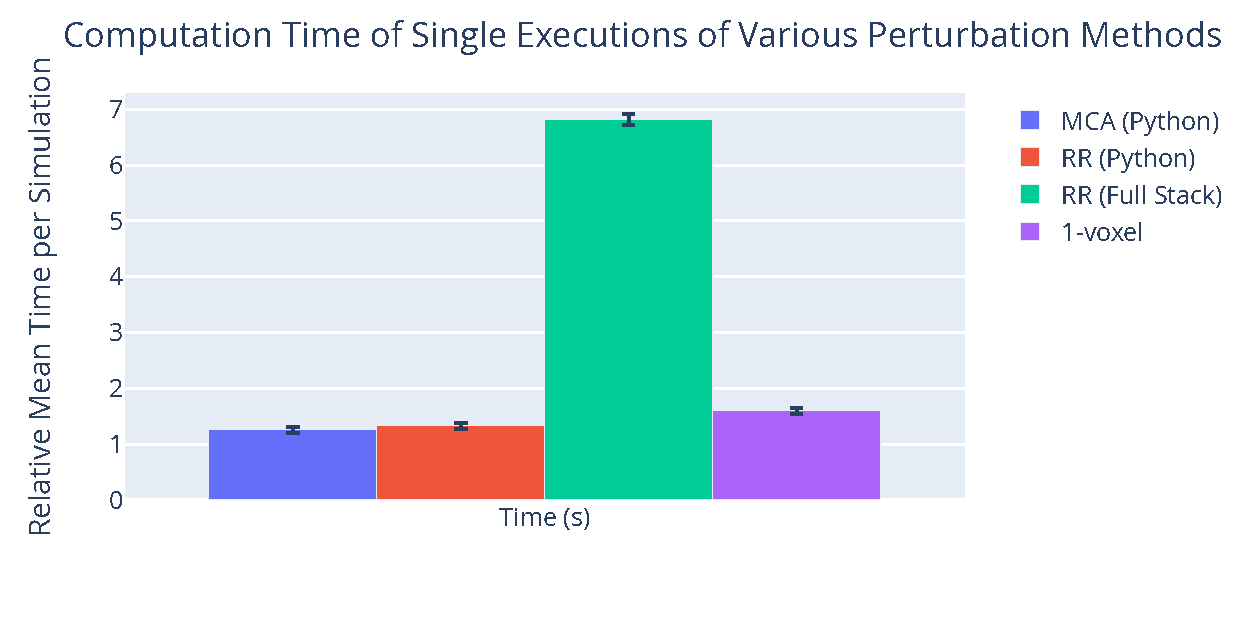
\includegraphics[width=\linewidth]{figures/fig6_timing.pdf}}
\caption{\textbf{Computation time for each perturbation method}. Shown in relative
time to the reference execution, plotted is the average execution time for the
perturbation methods. MCA and RR (Python) have a small increase in computation
time per run, as few floating point operations were instrumented in these settings.
The RR (Full Stack) method has nearly a $7 \times$ slowdown. In this case, all
floating point operations were instrumented, but the slowdown of less than the
estimated $100 \times$ would suggest that the bulk of computation time is not spent
on floating point arithmetic. The $1$-voxel implementations had a minor slowdown due
to the regeneration of data prior to pipeline execution. In every case, the
real-world slowdown is $S \times$ larger, where $S$ is the number of simulations,
in this case $100$.}
\label{fig5:timing}
\end{figure}

As the significance of RR (Full Stack) perturbation was highly variable across participants, this technique could also
be used for automated quality control, flagging high-variance subjects for further inspection or exclusion from
analyses. From the top level, inspecting the regional degradation of signal across these perturbations as shown in
Fig.~\ref{fig3:exploration}, researchers could lead a targeted interrogation of their raw datasets to identify
underlying causes of signal loss. Conversely, investigating which low-level BLAS operations contribute to the observed
instabilities will allow researchers to clarify the link between ill-conditioning and so-called ``bad data'' directly
within their pipelines. Upon characterizing this relationship it would be valuable to identify the point (if any) at
which targeted N-voxel perturbations become equivalent to MCA-induced variability, bridging the Uncertainty
Quantification and Numerical Analysis approaches.

The differences observed when performing $1$-voxel perturbations were often comparable in magnitude to the variation
introduced across Operating Systems. As OS noise is not controlled and may differ greatly among distributions, package
updates, etc., it is likely an insufficiently descriptive evaluation method, and should be used as a reference
alongside others. The level of control made available through $1$-voxel perturbations in terms of both locality and
strength of noise makes it a flexible option that could potentially be used to target known areas of key importance for
subsequent analyses. Due to the fact that these perturbations introduce a minor change to input images, this method
could also be used for estimating global pipeline stability in a classical sense (i.e. conditioning).

While each of the perturbation modes showed distinct differences with respect to the magnitude and continuity of their
induced deviations, Fig.~\ref{fig4:structural_variances} illustrates that the structure of these deviations was also
highly variable across both perturbation method and data. This suggests different applications and use cases for each
perturbation method. While MCA and RR Python implementations impact connectomes globally, these could be applied to
generate synthetic datasets. Full Stack RR is highly variable with respect to dataset, suggesting possible applications
in quality control, granted further work is performed to more fully understand the effect observed between this and the
Python-only case. Both $1$-voxel methods add noise locally, and can test the sensitivity of specific pipeline
components or regions of interest to variation. Other methods, such as automatic differentiation, could also be
explored as possible avenues leading towards an understanding of the end-to-end conditioning of pipelines.

In addition to generating unstable derivatives which could be looked at or analyzed independently, this type of
perturbation analyses enables the aggregation of derivatives. As is summarized in Fig.~\ref{fig5:aggregation_methods},
the method by which graphs or edges are aggregated can drastically change the construction of resulting graphs. While
the mean and max (i.e. $100^{th}$ percentile) methods both retain all edges that have appeared in even a single graph,
the minimum ($0^{th}$ percentile) and other low-percentile aggregations require a stricter consensus of edges for
inclusion in the final graph. A benefit of performing multiple aggregations is the composition of graphs with complex
edge composition, such as the most volatile edges, as is shown in the final column of
Fig.~\ref{fig5:aggregation_methods}. While the binary edge count in the composite graphs varies in each of these
methods, it is unclear how derived graph statistics will be affected, and that remains an exciting question for further
exploration.

From a resource perspective, each of the perturbation methods evaluated requires multiple iterations to get a sense of
the pipeline stability or build aggregates, here taken as $100$ iterations. Though the MCA-based methods have the
obvious disadvantage of extra computational overhead within each execution cycle of the pipeline, the noise-injection
methods do not increase the computation time for a single pipeline execution itself but in this case added
computational burden for the generation of synthetic data dynamically, reducing the redundancy of stored images on
disk. While Verificarlo has been demonstrated to account for an approximately $100 \times$ slowdown in floating
point operations~\cite{Denis2016-wo}, the largest slowdown observed in this pipeline is approximately a factor of $7$,
as shown in Fig.~\ref{fig5:timing}. This suggests that the bulk of time on CPU for this pipeline is not spent on
floating point operations, but perhaps other operations such as looping, data access, or manipulation of information
belonging to other data types. While this slowdown is observed for the the Full Stack implementation, the Python-only
implementation is negligibly slower than the reference execution, suggesting that even fewer of the floating point
logic is directly written in Python. The slowdown in the $1$-voxel setting is of a similar scale to that of the
Python-only implementation, with the slowdown likely caused by the addition of 2 read and 1 write operations to the
pipeline's execution (reading of simulation parameters and original image, application of simulation, and subsequent
writing of perturbed image to temporary storage). Note that the figures shown in Fig.~\ref{fig5:timing} are for a
single simulation, and real relative CPU time in each case would be $100 \times$ larger for the experimental
application of these methods.

The work presented here demonstrates that even low order computational models such as a 6-component tensor used in
diffusion modelling are susceptible to noise. This suggests that stability is a relevant axis upon which tools should
be compared, developed, or improved, alongside more commonly considered axes such as accuracy/biological feasibility or
performance. The heterogeneity observed across participants clearly illustrates that stability is a property of not
just the data or tools independently, but their interaction. Characterization of stability should therefore be
evaluated for specific analyses and performed on a representative set of subjects for consideration in subsequent
statistical testing. Additionally, identifying how this relationship scales to higher-order models is an exciting next
step which will be explored. Finally, the joint application of perturbation methods with more complex post-processing
bagging or signal normalization techniques may lead to the development of more numerically stable analyses while
maintaining sensitivity that would be lost in traditional approaches such as smoothing.

\section{Conclusion}\label{SCM}
All pipeline perturbation methods showed unique non-zero output noise patterns in low-order diffusion modeling,
demonstrating their viability for exploring numerical stability of pipelines in neuroimaging. MCA and RR (Python)
instrumented pipelines resulted in a wide range of variability, sometimes equivalent to subject-level differences, and
are recommended as possible methods to estimate the lower-bound of stability of analyses, generation of synthetic
datasets, and possible identification of Python-introduced critical branch points. RR (Full Stack) perturbations
resulted in continuously distributed connectomes that were highly variable across datasets, ranging from negligible
deviations to complete regional signal degradation. We provisionally recommend the use of RR (Full Stack) noise for
automated quality control and identifying global pipeline stability. While $1$-voxel methods result in considerably
smaller maximum deviations than the MCA-based methods, they are far more flexible and enable evaluating the sensitivity
of pipelines to minor local data perturbations. While the MCA-based methods are more computationally expensive than
direct $1$-voxel noise injections, the slowdown was found to be less significant in practice than the $100 \times$
scaling factor estimated per floating point operation, presumably due to a significant portion of the pipeline
computation time being spent on data management or string and integer processing rather than the constant use of
floating point arithmetic.

In all cases, while tool instrumentation enables the parallelized simulation of a particular set of instructions, the
aggregation of the simulated graphs is an essential component of the downstream analyses both when exploring the nature
of instabilities or developing inferences upon the pipeline's derivatives. We recommend a percentile approach to
aggregation, where the threshold can be adjusted based on the desired robustness of the resulting graphs. An advantage
of percentile approaches is also that composite aggregates can be formed, isolating edges based on their prevalence
across simulations. Further exploration of the distribution of perturbed results should be performed to conclude on the
relevance of the aggregation used, as the desired aggregate should be close to the expected value of the distribution.

While both MCA and random-injection simulations are computationally expensive in that they require the evaluation of
many simulations, they provide an opportunity to characterize processing modes that may emerge when analyzing either
noisy datasets or unstable tools. This work also highlighted an important relationship between the noise properties of
an incoming dataset and the tool, validating the need to jointly evaluate the stability of tool--dataset combinations.

Where this work demonstrates a range of numerical variation across minor changes in the quality of data or computation,
it does not address the analytic impact of these deviations on downstream statistical approaches. This open question,
as well as the relative impact of normalization techniques on this process, present avenues for research which will
more clearly place these results in a biologically relevant context, allowing characterization of the functional impact
of the observed instabilities.

\subsection*{Acknowledgments}
This research was enabled in part by support provided by Calcul Quebec
(\href{http://www.calculquebec.ca}{http://www.calculquebec.ca}) and Compute Canada (\href{http://www.computecanada.ca}{http://www.computecanada.ca}). We would also
like to thank Dell and Intel for their collaboration and contribution of computing infrastructure. The authors would
also like to thank their reviewers for thoughtful and insightful comments and suggestions.

%----------------------------------------------------------------------------------------
%	REFERENCE LIST
%----------------------------------------------------------------------------------------
\phantomsection
{\small 
\bibliographystyle{IEEEtran}
\bibliography{chapter2}
}
%----------------------------------------------------------------------------------------
\end{document}
